\chapter{The LHCb experiment}
\label{cap:LHCb}

\section{The Large Hadron Collider}

\begin{figure}[t]
	\centering
	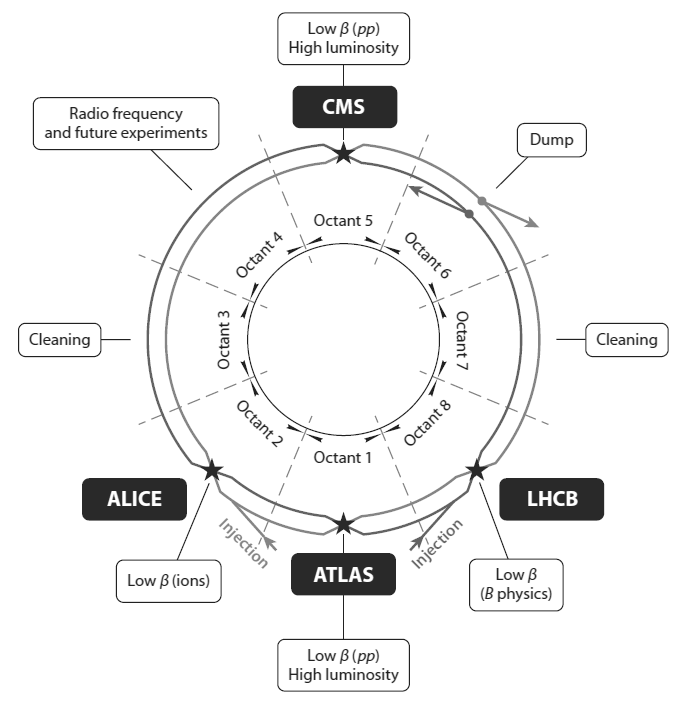
\includegraphics[width=.6\textwidth]{graphics/02-lhcb/lhc_diagram.png}
	\caption[LHC schematic layout.]{Layout of the Large Hadron Collider with its four main experiments \cite{doi:10.1146/annurev-nucl-102010-130438}.}
	\label{fig:2:lhc_diagram}
\end{figure}

At the moment of writing, the Large Hadron Collider (LHC for short) is the largest and most powerful particle collider in the world.

Da dire:
\begin{itemize}
	\item Two counterrotating rings
	\item CERN (cos'è)
	\item Proton-proton
	\item Approvato 1994 in due fasi center-of-mass collision energy 10 -> 14 TeV, 1996 in fase singola a 14 TeV
\end{itemize}


\section{The LHCb experiment and detector}

\begin{figure}[t]
	\centering
	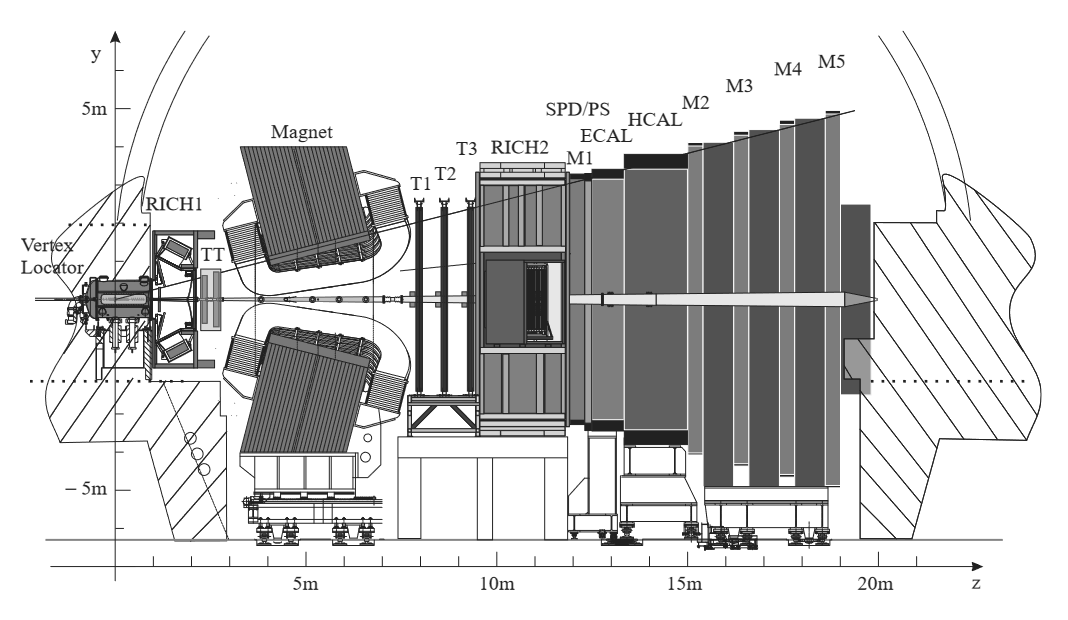
\includegraphics[width=\textwidth]{graphics/02-lhcb/lhcb_diagram.png}
	\caption[LHCb detector side view.]{Side view of the LHCb detector used for LHC Run 1 and 2 \cite{Antunes-Nobrega:630827}.}
	\label{fig:2:lhcb_diagram}
\end{figure}

LHCb (the \textit{b} stands for \textit{beauty}\footnote{Before settling on the names \textit{top} and \textit{bottom} for the third generation of quarks, the names \textit{truth} and \textit{beauty} were among those proposed. While they never gained enough momentum in the scientific community, echoes of the failed nomenclature are still present in heavy quark vocabulary, for instance in the alternative name \textit{truth} for the \textit{topness} flavour number mentioned in Section \ref{sec:flavour-physics}, as well as in the official name for the LHCb experiment.}) is one of the four main experiments at the LHC.

Elenca i successi.

\label{info:LHCb_system}
RICORDA DI DIRE IL SISTEMA DI COORDINATE!
Non usare questo, che è preso da online:
A right-handed coordinate system is defined centred on the interaction point, with z along the beam axis and y pointing upwards.

\subsection{Tracking}

\subsubsection{VELO}

\subsubsection{Tracker Turicensis}

\subsubsection{T stations}

\subsubsection{Track classification}

\begin{figure}[t]
	\centering
	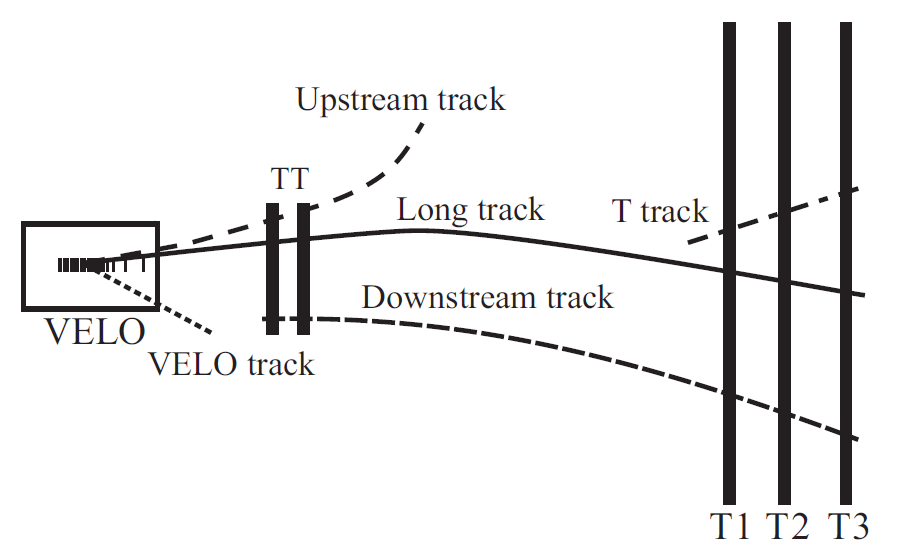
\includegraphics[width=.8\textwidth]{graphics/02-lhcb/Track_Definitions.png}
	\caption{A.}
	\label{fig:2:track_classification}
\end{figure}

Qui tutta la storia delle T track

\subsection{Particle identification}

\subsubsection{RICH}

\subsubsection{Calorimeter}

\subsubsection{Muon system}

\section{The LHCb data flow}
Qui trigger, track reconstruction e tutto il resto.

\section{LHCb detector upgrade for Run 3}

\begin{figure}[t]
	\centering
	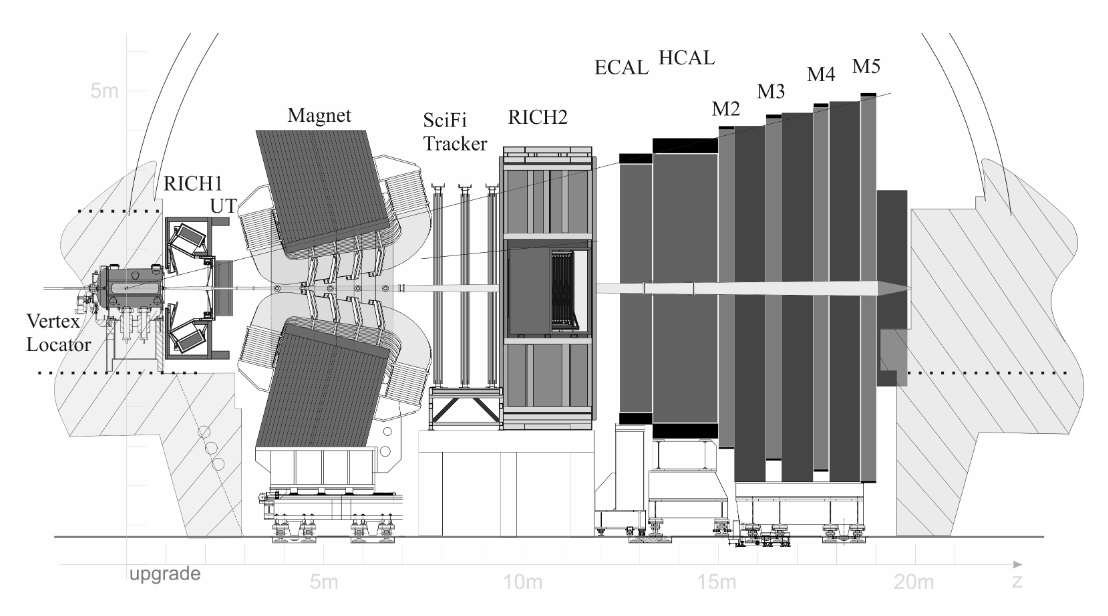
\includegraphics[width=\textwidth]{graphics/02-lhcb/lhcb_diagram_run3.png}
	\caption[LHCb detector side view.]{Side view of the upgraded LHCb detector for future usage in LHC Run 3 \cite{Piucci_2017}.}
	\label{fig:2:lhcb_diagram_run3}
\end{figure}

\section{Data}
Non so se vada qui ma da qualche parte deve andare.